\documentclass[5p,times,numbers,authoryear]{elsarticle}

\usepackage{ctex}
\usepackage{lineno}%,hyperref}
\usepackage[colorlinks,citecolor=blue]{hyperref}

\usepackage{graphics}
\usepackage{graphicx}
\usepackage{subfigure}
\usepackage{enumitem}
\usepackage{helvet}
\usepackage{courier}
\usepackage{diagbox}
\usepackage{amsmath}
\usepackage{multirow}
\usepackage{booktabs}
\usepackage{makecell}
\usepackage{amssymb}
\usepackage{threeparttable}
\usepackage[justification=centering]{caption}
\usepackage[linesnumbered,ruled,vlined,commentsnumbered]{algorithm2e}
\usepackage{color}
\usepackage{xcolor}
\usepackage{colortbl}
\usepackage{float}
\usepackage{bm}
\usepackage[normalem]{ulem} % use normalem to protect \emph
\newcommand\hl{\bgroup\markoverwith
  {\textcolor{yellow}{\rule[-.5ex]{2pt}{2.5ex}}}\ULon}

\usepackage{hyperref}
\usepackage{breakurl}

\newtheorem{definition}{Definition}
\def\boxend{\hspace*{\fill} $\Box$}
\newcommand{\comment}[1]{}
\renewcommand{\multirowsetup}{\centering}

\journal{Computers in Human Behavior}

\usepackage{appendix}

\begin{document}

\begin{frontmatter}

\title{Stress-Buffering Pattern of Positive Events on Adolescents: \\
An Exploratory Study Based on Social Networks}


\begin{abstract}
Stress is viewed as the leading cause of mental health issues. 
Positive events, however, could act as a buffer against stress. 
Since the stress-buffering effects of positive events in previous studies were mainly examined by subjective self-reporting, continuous tracking research at individual behavioral levels still remains to be explored. 
In this study, we collected microblogs (n=27,346) from a group of high school students  (n=500) to examine the relationship between positive events and stress-buffering patterns at both the content and behavioral levels. 
Through a pilot study of scheduled exam intervals under two situations, namely, 
1) existing neighboring positive scheduled events (n=75) and 2) no neighboring positive events,
we found that students taking exams with neighboring positive events appeared to exhibit less intense stress and more stable stress fluctuations. 
Most students talked less about exams when positive events occurred nearby, at a lower frequency and a lower ratio. 
Hypothetical tests for stress-buffering effects of positive events and monotonic changes in the stress intensity under the impact of positive events were further conducted based on automatically extracted positive events (n=1,914) from the microblogs. 
The results showed that the stress-buffering effects of positive events were closely correlated with adolescents�� stress-change modes, microblog linguistic expressions, and posting behaviors.
The occurrence of positive events was verified to offset the impact of stressor events through talking about positive topics at the same time.
Adolescents tended to post more forwarded microblogs, more positive microblogs and less stressful microblogs when positive events appeared; 
however, the total frequency of microblogs did not appear to change significantly under the impact of positive events.
The study also showed that positive events buffered monotonic changes in stress intensity caused by stressor events.
Based on these theoretical findings, the stress-buffering patterns around positive events were further incorporated for stress prediction in adolescents, and the predictive performance was improved. 
This study could inform the use of social networks to estimate and track mental health transition in adolescents under stress. 
The theoretical and practical implications, limitations of this study and future work are discussed.
\end{abstract}

\begin{keyword}
stress-buffering effect, positive events, microblogs, adolescents
\end{keyword}
\end{frontmatter}


\section{Introduction}
\emph{Motivation}: Life is always full of ups and downs.
Accumulated stress could drain inner resources,
leading to psychological maladjustment, depression and even suicidal behaviors \citep{Nock2008Suicide}.
Compared to adults, young people exhibit high levels of stress due to their immature inner status and lack of experience \citep{older}.
According to the latest report released by the American Psychological Association in 2018,
91\% of young adults had experienced physical or emotional symptoms due to stress in the past month compared to 74\% of adults \citep{APA2018}.
More than 30 million Chinese adolescents suffer from psychological stress,
and nearly 30\% of them are at a risk of depression \citep{ChinaTeen2019}.
Stress-induced mental health problems are becoming an important social issue. 
%1.����ѹ�����������

On the other hand, positive life events, such as satisfying social interactions,
excellent academic performance and pleasant entertainment activities, could exert protective effects on emotional distress in both direct and indirect ways by '\emph{buffering}'~\citep{Shahar2002Positive, Cohen2010Positive}, with respect to physiological, psychological, and social coping resources~\citep{Cohen1984Positive,Needles1990Positive}.
Researchers indicated that positive events mitigated the relationship between negative events and maladjustment in samples of adolescents experiencing family transitions~\citep{Doyle2003Positive}.
The written expression of positive feelings could prompt increased cognitive reorganization in undergraduate students~\citep{Coolidge2009A}.
Positive events have also been linked to medical benefits, such as improved mood, serum cortisol levels, and lower levels of inflammation and hypercoagulability~\citep{Caputo1998Influence,Jain2010Effects}.
Thus, tracking the state of the stress-buffering effect is important for understanding the mental status of stressed individuals.
%2.�����¼����Ի�������ѹ����

\emph{Existing solutions}:
Previous studies have focused on measuring positive events and stress-buffering states after events through questionnaires, including the Hassles \& Uplifts Scales~\citep{Kanner1981Comparison}, the Interpretation of Positive Events Scale~\citep{Alden2008Social},
the Adolescent Self-Rating Life Events Checklist~\citep{Jun2008Influence} and the Perceived Benefit Scales~\citep{Mcmillen1998The}.
Recently, scholars have demonstrated the feasibility to sense and predict users' stress from social networks~\citep{XueUbicomp13,Xue2014Detecting,Lin2014User,Li2015When,Li2015Predicting,Li2015Using,
Li2017Analyzing,Li2017Exploring} through content (linguistic text, emoticons and pictures) and behavioral (abnormal posting time and comment/response actions) measures.

If we view the aforementioned traditional studies as static sensing of stress-buffering, this study approaches the stress-buffering as a dynamic process and aims to find a solution at both the microblogging-content and behavioral levels under the hypothesis that the occurrence of positive events can be reflected in adolescents' microblogs.
Self-report investigations are susceptible to many factors,
such as social pressure and pressure from measurement scenarios, but microblogging characteristics at the behavioral level are objective expressions that can assist in identifying content characteristics.

Another difference from the previous studies lies in that, despite the unique advantages of social networks over traditional survey methods in offering self-expressed content and behavioral information, previous microblog-based studies stopped at the analysis of stress, and none went further to capture positive events that may play a key role in adolescents' stress-coping mechanisms.
For example, ��hiking tomorrow�� might simultaneously occur and be expressed in microblogs with ��failing the exam today��.
If do not know anything about positive events, is the unilaterally detected stress the real stressful state of the current youth?
Understanding stress-buffering patterns of positive events is helpful in precisely predicting and guiding
adolescents who are coping with stress.

\emph{Our work}:
To this end,
this paper studies adolescent stress from the dual perspective of stress generation and stress-buffering
and views stress as the superposition effect of stressors and positive events.
By investigating the connection between positive events and stress changes
reflected through adolescents' microblogging content and behaviors,
we discover stress-buffering patterns of positive events and further predict future stress under such mitigation.
Exploiting stress-buffering effects of positive events
is also advantageous in handling the confusing situation
whether an adolescent who doesn't express stressful information from microblogs is actually under stress.

However, capturing the stress-buffering process of positive events is not a trivial task.
Three fundamental challenges need to be addressed:
1) What are the criteria for depicting stress-buffering effects?
2) What is the latent connection between positive events and adolescents' stress-buffering reflections in microblogs?
3) How can identify positive events and their impact interval be extracted from microblogs?

A pilot study was first conducted on the microblog data (n=27,346) of a group of high school students (n=500) associated with the school's positive scheduled events (n=75) and stressor events (n=122).
Stressful intervals were divided into two comparative categories: intervals impacted by positive scheduled events (denoted by U-SI, n=259) and intervals not impacted by positive scheduled events (denoted by SI, n=518).
After observing the posting behaviors and microblog content of the stressed students in both the SI and U-SI groups,
several implications were discussed to guide the next step of the study.
Motivated by the implications of the pilot study, we modeled the connection between positive events and adolescents' stress-buffering reflections
as the statistical difference in two comparative situations SI and U-SI.
Three groups of measures were adopted to depict adolescent stress buffering at the period level:
stress-change modes, linguistic expressions and posting behaviors.
Monotonic changes in stress intensity buffered by positive events were measured in temporal order.
As an exploration,
according to the occurrence of automatically extracted positive events,
we covered the stress-buffering effects into each time unit and integrated such an effect into the stress prediction model.

In this paper,
to automatically extract positive events,
we built upon and extended previous stress and event detection works.
A Chinese linguistic parser model was applied to extract positive events in the linguistic structure
\emph{[type, (act, doer, description)]}.
We followed the categorization of adolescents' positive events in six dimensions (entertainment, school life, romantic, peer relationships, self-cognition and family life) and extended the SC-LIWC lexicons into 2,606 phases.
Stressful intervals (SI) and stressful intervals impacted by positive events(U-SI) were identified according to their temporal order.

The rest of the paper is organized as follows.
We review the literature in section \ref{sec:related} and introduce the pilot study in section \ref{sec:obs}.
The procedure for extracting positive events is presented in section \ref{sec:frame1}.
The connection between positive events and adolescents' stress buffering from microblogs are discussed and modeled in section \ref{sec:frame2}.
We present the experimental results in section \ref{subsec:experiment} and extend the study to integrating stress-buffering patterns into future stress prediction in section \ref{subsec:predict}.
Future work is discussed in section \ref{sec:conclude}.

\section{Literature Review}
\label{sec:related}
\subsection{Stress-buffering Function of Positive Events}
%3.����ɱ���¶��У�ѹ���ĵ�������
Positive events have been verified as protective factors against daily stress~\citep{Ong2006Psychological,Bono2013Building}, loneliness~\citep{Chang2015Loneliness}, suicide~\citep{Evan2014Social} and depression~\citep{Santos2013The}.
Through exploring naturally occurring daily stressors, \citep{Ong2006Psychological} found that over time,
the experience of positive emotions functions to assist high-resilient individuals to recover effectively from daily stress.
Through a three-week longitudinal study, \citep{Bono2013Building} examined the correlation between employee stress and health and positive life events, and concluded that naturally occurring positive events are correlated with decreased stress and improved health.
\citep{Chang2015Loneliness} investigated the protective effect of positive events in a sample of 327 adults, and found that the positive association between loneliness and psychological maladjustment was found to be weaker for those who experienced a high number of positive life events, as opposed to those who experienced a low number of positive life events.
This is assistant with the conclusion made by \citep{Evan2014Social} that positive events acted as protective factors against suicide individually and synergistically when they co-occurred,
by buffering the link between important individual differences risk variables and maladjustment.
In the survey made by \citep{Santos2013The},
strategies of positive psychology were also checked as potentially tools for the prophylaxis and treatment of depression, helping to reduce symptoms and for prevention of relapses.

%2.�����¼����õ����ַ�ʽ
The protective effect of positive events was hypothesized to operate in both directly (i.e., the more positive events people experienced, the less stress they perceived)
and indirectly ways by \emph{'buffering'} the effect of stressors ~\citep{Cohen2010Positive,Shahar2002Positive},
with respect to physiological, psychological, and social coping resources ~\citep{Cohen1984Positive, Needles1990Positive}.
%1.�����¼��������������棺�����������ۣ�������⣬�����»����¼�
\citep{Folkman2010Stress} identified three classes of coping mechanisms that were associated with positive emotion during chronic stress: positive reappraisal, problem-focused coping, and the creation of positive events.
%4. ����������¼��������ĵ�������
Due to the immature inner status and lack of experience,
adolescents exhibit more sensitive to stressors
(i.e., exams, heavy homework, isolated by classmates, family transitions),
living with frequent, long-term stress~\citep{older}.
In this situation,
positive events could help reinforce adolescents' sense of well-being~\citep{Coolidge2009A},
restore the capacity for dealing with stress~\citep{Doyle2003Positive},
and also have been linked to medical benefits, such as improving mood, serum cortisol levels, and lower levels of inflammation and hyper coagulability \citep{Jain2010Effects,Caputo1998Influence}.
The present study will be based on the consensus conclusions from the above studies.

To assess the stress-buffering effect of positive events,
scholars conducted many studies based on self-support methods.
For example,
\citep{Kanner1981Comparison} conducted Hassles \& Uplifts Scales,
and concluded that the assessment of daily hassles and uplifts might be a better approach to the prediction of adaptational outcomes than the usual life events approach.
To measure negative interpretations of positive social events,
\citep{Alden2008Social} proposed the Interpretation of Positive Events Scale, and analyzed the relationship between social interaction anxiety and the tendency to interpret positive social events in a threat-maintaining manner.
\citep{Mcmillen1998The} proposed the Perceived Benefit Scales as the new measures of self-reported positive life changes after traumatic stressors, including lifestyle changes, material gain, increases in self efficacy, family closeness, community closeness, faith in people, compassion, and spirituality.
Specific for college students,
\citep{Jun2008Influence} investigated in 282 college students using the Adolescent Self-Rating Life Events Checklist, and found that the training of positive coping style was of great benefit to improve the mental health of students.
The above explorations based on self-report investigations
were difficult to exclude interference from external factors (i.e., social appreciation, pressure from measurement scenarios).
Meanwhile, due to the lack of manpower and effective scientific methods,
most scholars relied on a limited number of measurements,
thus continuous measurements of stress-buffering process were difficult to carry out.

\subsection{Measures and Stress Analysis from Social Networks}
As billions of adolescents are recording their life through social networks (e.g., micro-blog, Twitter, Facebook),
researchers explored to apply psychological theories into social network based data mining techniques,
thus to better understand user' psychological status from the self-expressed public data source.
Multiple content and user behavioral measures have been proven effective in user mental health analysis,
including time series curve analysis of stress~\citep{Li2015When,Li2015Using}, topic words~\citep{XueUbicomp13}, abnormal posting time~\citep{Xue2014Detecting},
online shopping behaviors~\citep{DBLP:conf/apweb/Zhao0XLF16},
human mobility features~\citep{DBLP:conf/dasfaa/JinXLF16}, comment/response actions~\citep{Liang2015Teenagers}
and high dimensional multimedia features~\citep{Lin2014User}.
For example,
\citep{XueUbicomp13, Xue2014Detecting} proposed to detect adolescent stress from single post utilizing machine learning methods by extracting stressful topic words, abnormal posting time, and interactions with friends.
\citep{Lin2014User} constructed a deep neural network to combine the high-dimensional picture semantic information into stress detecting.
Based on the stress detecting result,
\citep{Li2015Predicting}\cite{Li2015Using}\cite{Li2015When} adopted a series of multi-variant time series prediction techniques (i.e., Candlestick Charts, fuzzy Candlestick line, Seasonal Autoregressive Integrated Moving Average model) to predict future stress trend.
Taking the linguistic information into consideration,
\citep{Li2017Exploring} employed a Nonlinear autoregressive with External Input Neural Network to predict a teen's future stress level referred to the impact of co-experiencing stressor events of similar companions.
\citep{Li2017Analyzing} proposed to detect stressor events from microblog content
and analyze stressful intervals based on posting rate.
All above studies focused on the discussion of stress detection on social networks.
This paper starts from a completely new perspective,
and focuses on the stress-buffering effect of positive events in adolescents' stress coping process.
Thus we push forward the study from how to find stress to the next more meaningful stage: how to cope with stress.

\subsection{Correlation Analysis Models for Multivariate Time Series}
Basic correlation analysis models on time series focused on univariate data have been well studied.
As the most widely adopted model,
the Pearson correlation analysis \cite{Cohen1988Statistical} measures the linear correlation between two variables $X$ and $Y$.
One inevitable defect of Pearson correlation is its sensitivity to outlier values.
To overcome such drawback,
Spearman Rank correlation \cite{C1987The}
and Kendall Rank correlation \cite{Mcleod2011Kendall}
were proposed based on Pearson correlation.
While Pearson correlation estimates linear relationships,
Spearman correlation estimates monotonic relationships (whether linear or not),
and are calculated as the Pearson correlation between the rank values of two variables.
The Kendall Rank correlation mainly assesses the similarity of the orderings of the data when ranked by each of the quantities.
The above correlation models are usually used to estimate relationship between single-dimensional variables,
and cannot be adopted directly in social network based scenario.

For multivariate time series analysis,
two-sample based models were widely adopted.
Such kind of models were deduced to check whether two samples come from the same underlying distribution,
which was assumed to be statistically unknown.
Correspondingly,
various kernel \citep{Sch2006A} and distance-based models \citep{Schilling1986Multivariate} were proposed.
\citep{Sch2006A} proposed to transform the distance between two variables and nearest neighbors into a reproducing kernel hilbert pace, and solve the problem using Maximum Mean Discrepancy.
\citep{Schilling1986Multivariate} adopted the $r$-nearest neighbor based model to partition two set of event driven time series data.
The global proportion of the right divided neighbors were calculated to estimate whether there existed statistically difference between the two sets.
This paper adopted the $r$-nearest neighbor based two-sample model in our problem,
thus to measure the distance and correlation between two multi-dimension variables depict
the stress-buffering patterns of positive events.

\section{Data Observation: A Pilot Study on the Stress-buffering Effect of School Scheduled Positive Events}
\paragraph{Microblogs} Microblogs of students coming from Taicang High School,
were collected from January 1st, 2012 to February 1st, 2015. 
We filtered out 124 active students according to their posting frequency from over 500 students,
and collected their microblogs throughout the whole high school career.
Totally 29,232 microblogs were collected in this research,
where 236 microblogs per student on average, 1,387 microblogs maximally and 104 posts minimally.
To protect the privacy, all usernames were anonymized during the experiment. 

\paragraph{Scheduled events} The list of weekly scheduled school events, 
with detailed description involved in the event (grade, exact start and end time), 
were collected from the school's official website\footnote{http://stg.tcedu.com.cn/col/col82722/index.html} from February 1st, 2012 to August 1st 2017.
There were 122 stressor events and 75 positive events in total. 
Examples of scheduled positive and stressor events in high school life are listed shown in Table~\ref{tab:example}.
There were 2-3 stressor events and 1-2 positive event scheduled per month in current study.
Figure~\ref{fig:example} shows three examples of a student's stress fluctuation during three mid-term exams,
where the positive event \emph{campus art festival} was scheduled ahead of the first exam (\emph{example a}),
the positive event \emph{holiday} happened after the second exam (\emph{example b}),
and no scheduled positive event was found nearby the third exam (\emph{example c}).

\begin{table}[H]
\caption{\small{Examples of school scheduled positive and stressor events.}}
\label{tab:example}
\resizebox{.45\textwidth}{9mm}{
\small{
\begin{tabular}{cccc}
\toprule
Type & Date	& Content	& Grade	\\
\midrule
stressor event & 2017/4/16 & \emph{first day of mid-term exam} & grade1,2\\
positive event & 2016/11/5 & \emph{campus art festival} & grade1,2,3\\
\bottomrule
\end{tabular}
}
}
\end{table}

\begin{figure}[H]
\centering
\includegraphics[width=\linewidth]{figs/exampleWave.eps}
\caption{\small{Examples of school scheduled positive events, stressful events, and a student's stress fluctuation}}
\label{fig:example}
\end{figure}

To further observe the effect of positive events on stressed students,
we collected all stressful intervals surround the scheduled exams over the 124 students during their high school career
applying the interval detection method in ~\citep{Li2017Analyzing}. 
For each student, we divided all stressful intervals into two sets: 
1) In the original sets, stress was caused by a stressor event, lasting for a period,
and no other intervention (namely, positive event) occured.
We called the set of such stressful intervals as \textbf{SI};
2) In the other comparative sets,
the stressful interval was impacted by a positive event(i.e., uplifts),
we called the set of such stressful intervals as \textbf{U-SI}.
Thus the difference under the two situations (sets) could be seen as the stress-buffering effect
conducted by the positive event. 
We identified 518 exam related stressful intervals (SI)
and 259 stressful intervals impacted by four typical scheduled positive events (U-SI)
('practical activity', 'new year party', 'holiday', 'sports meeting') from the students' microblogs. 
Five measures during the above two conditions were considered:
the \emph{accumulated stress}, the \emph{average stress} (per day), the \emph{length of stressful intervals},
the \emph{frequency of academic topic words}, and the \emph{ratio of academic stress among all types of stress}.
.......... 
Examples of topic words for each type of positive event were listed in table \ref{tab:keyWords}. 
Examples of academic related keywords were listed in table \ref{tab:studyWords}. 
%topic to further study
The average value of each measure over all eligible slides was calculated. 
Since our target was to track the stress-buffering effect of positive events for students under stress, 
based on previous research~\cite{XueUbicomp13}, 
we detected the stress level (ranging from 0 to 5) for each post.
For each student,
the stress value per day was aggregated by calculating the average stress of all posts. 
The positive level of each post was identified based on the frequency of positive words. 

\begin{table*}
\centering
\caption{\small{Examples of topic words for positive events.}}
\label{tab:keyWords}
\small{
\begin{tabular}{lll}
\toprule
dimension & example words & total \\ \midrule
\emph{entertainment}  & hike, travel, celebrate, dance, swimming, ticket, shopping, air ticket, theatre, party, Karaoke,& 452\\
                      & self-driving tour, game, idol, concert, movie, show, opera, baseball, running, fitness, exercise & \\
\emph{school life}    & reward, come on, progress, scholarship,admission, winner, diligent, first place, superior & 273\\
				      & hardworking, full mark,  praise, goal, courage, progress, advance, honor, collective honor& \\
\emph{romantic}       &  beloved, favor, guard, anniversary,  concern, tender, deep feeling, care, true love, promise, & 138\\
				      & cherish, kiss, embrace, dating, reluctant, honey, sweetheart, swear, love, everlasting, goddess &\\
\emph{pear relation}  & listener, company, pour out, make friends with, friendship, intimate, partner, team-mate, brotherhood& 91\\
\emph{self-cognition} & realize, achieve, applause, fight, exceed, faith, confidence, belief, positive, active, purposeful & 299\\
\emph{family life}    & harmony, filial, reunite, expecting, responsible, longevity, affable, amiability, family, duty & 184\\
\bottomrule
\end{tabular}}
\end{table*}

\begin{table}[h]
\centering
\caption{\small{Examples of academic related keywords.}}
\label{tab:studyWords}
\small{
\begin{tabular}{c}
\toprule
exam, fail, review, score, test paper, rank, pass, math, chemistry\\
homework, regress, fall behind, tension, stressed out, physics,\\
nervous, mistake, question, puzzle, difficult, lesson, careless\\
\bottomrule
\end{tabular}
}
\end{table}

\subsection{Results}
As shown in figure~\ref{fig:frequency},
comparing each measure of scheduled exam intervals under the two situations:
1) existing neighbouring positive events (U-SI) or 2) no neighbouring scheduled positive events (SI),
we found that students during exams with neighbouring positive events exhibited less average stress intensity
(78.13\% reduction in average stress, 95.58\%  reduction in cumulative stress)
and shorter duration of stress intervals (23.30\% reduction).
Further, the frequency of academic topic words (table \ref{tab:studyWords} for examples)
and the ratio of academic stress in each interval were calculated.
Results in figure~\ref{fig:frequency} shows that most students talked less about the upcoming or just-finished exams when positive events happened nearby,
with lower frequency (84.65\% reduction) and lower ratio (89.53\% reduction). 
The statistic result shows clues about the stress-buffering effect of scheduled positive events,
which is constant with the psychological theory ~\citep{Cohen1984Positive, Cohen2010Positive, Needles1990Positive},
indicating the reliability and feasibility of the microblog data set.
However,
this is an observation based on specific scheduled events,
and cannot satisfy the need for automatic, timely, and continuous perception of stress-buffering process.
Therefore, next, we will propose a framework to automatically detect positive events and its impact interval.
Based on this,
the relationship between stress-buffering effect of automatically extracted positive events and
microblog characteristics will be discussed.

\begin{figure}[h]
\centering
\includegraphics[width=0.8\linewidth]{figs/obnew-color.eps}
\caption{\small{Comparing students' stress during exam intervals in two situations:
1) intervals affected by neighboring positive events (U-SI), 2) no positive events occurred nearby (SI)}}
\label{fig:frequency}
\end{figure}

\section{Framework}
We first introduce the procedure to extract positive event and its intervals from microblogs,
Based on this,
we present a statistical model to depict
the connection between positive events and adolescents' stress-buffering patterns through three groups of content and behavioral measures.
%Finally, a none-liner time series model was proposed to combine stress-buffering patterns into future stress prediction.
\subsection{Discovery of Positive Events from Microblogs}
\label{sec:frame1}
Let $u$ = $[type,\{doer, act,$ $description\}]$ be a positive event,
where the element \emph{doer} is the subject who performs the \emph{act},
and \emph{descriptions} are the key words related to $u$.
According to psychological scales ~\citep{Jun2008Influence,hassles},
adolescent positive events mainly focus on six dimensions,
as $\mathbb{U} =\{$ 'entertainment', 'school life', 'romantic', 'pear relationship', 'self-cognition', 'family life'$\}$. We constructed our lexicon for six-dimensional positive events from two sources.
The basic positive words are selected from the psychological lexicon C-LIWC (expectation, joy, love, surprise)~\citep{Tausczik2010The}.
Then we built six topic lexicons by expanding basic positive words from adolescent microblogs,
containing 452 phrases in 'entertainment',
273 phrases in 'school life',
138 phrases in 'romantic',
91 phrases in 'peer relationship',
299 phrases in 'self-recognition' and 184 phrases in 'family life', with totally 2,606 phrases,
as examples shown in table \ref{tab:topicWords}.
Additionally, we labeled \emph{doer} words (i.e., \emph{teacher}, \emph{mother}, \emph{I, we}) in positive lexicons.

\begin{table*}
\centering
\caption{\small{Topic words of six-dimensional positive events.}}
\label{tab:topicWords}
\small{
\begin{tabular}{lll}
\toprule
dimension & example words & total \\ \midrule
entertainment  & hike, travel, celebrate, dance, swimming, ticket, shopping, air ticket, theatre, party, Karaoke,& 452\\
                      & self-driving tour, game, idol, concert, movie, show, opera, baseball, running, fitness, exercise & \\
school life    & reward, come on, progress, scholarship,admission, winner, diligent, first place, superior & 273\\
				      & hardworking, full mark,  praise, goal, courage, progress, advance, honor, collective honor& \\
romantic       &  beloved, favor, guard, anniversary,  concern, tender, deep feeling, care, true love, promise, & 138\\
				      & cherish, kiss, embrace, dating, reluctant, honey, sweetheart, swear, love, everlasting, goddess &\\
pear relation  & listener, company, pour out, make friends with, friendship, intimate, partner, team-mate, brotherhood& 91\\
self-cognition & realize, achieve, applause, fight, exceed, faith, confidence, belief, positive, active, purposeful & 299\\
family life    & harmony, filial, reunite, expecting, responsible, longevity, affable, amiability, family, duty & 184\\
\bottomrule
\end{tabular}}
\end{table*}

\subsubsection{Linguistic Parser Model}
Positive events were identified through Chinese natural language processing platform \citep{Che2010}.
For each post, after word segmentation, we parsed each sentence to find its linguistic structure,
and then matched the main linguistic components with positive topic lexicons in each dimension.
The linguistic parser model was applied to identify the central verb of current sentence, namely the \emph{act}.
It constructed the relationship between the central verb and corresponding \emph{doer} and \emph{description} elements.
By searching these elements in positive topic lexicons,
the existence of positive events were identified.
Due to the sparsity of posts, the element \emph{act} might be empty.
\emph{Descriptions} were collected by searching all nouns, adjectives and adverbs.
Examples of positive events extracted from adolescents' microblogs are listed in table \ref{tab:uplifts}.
For the post 'Thanks all my dear friends hosting the party. Happiest birthday!!!',
it was processed as \emph{doer='friends', act = 'expecting', description = 'party'},
and \emph{type = 'entertainment'}.

\begin{table}
\begin{center}
\caption{\small{Extracted positive events from microblogs.}}
\small{
\begin{tabular}{|l|} \hline
I am really looking forward to the spring outing on Sunday now. \\
(doer:\emph{I}, act:\emph{looking forward}, description:\emph{spring outing})\\\hline
My holiday is finally coming [smile]. \\
(doer:\emph{My holiday}, act:\emph{coming}, description:\emph{[smile]})\\\hline
First place in my lovely math exam!!! In memory of it.\\
(description:\emph{first place, math, exam, memory})\\\hline
You are always here for me like sunshine. \\
(doer:\emph{You}, description:\emph{sunshine})\\\hline
Thanks all my dear friends hosting the party.
Happiest birthday!!!\\
(doer:\emph{friends}, act:\emph{thanks}, description:\emph{party, birthday})\\\hline
I know my mom is the one who support me forever, no matter \\
when and where. (doer:\emph{mom}, act:\emph{support})\\ \hline
Expecting Tomorrow' Adult Ceremony[Smile][Smile]~~\\
(act: \emph{expecting}, description:\emph{Adult Ceremony})\\\hline
\end{tabular}}
\label{tab:uplifts}
\end{center}
\end{table}

\subsubsection{Impact Intervals of Positive Events}
We followed and extended ~\citep{Li2017Analyzing} to identify the impact interval of each positive event to further study its stress-buffering pattern.
Splitting interval is a common time series problem, and here we identified the target interval in three steps.

Step1:
Extracted positive events, stressor events and filtered out candidate intervals.
For each candidate interval,
we set its length to more than 3 days and a maximum gap of 1 day between two neighboured stressed days.
Since the stress series detected from microblogs were discrete points,
loess method was adopted to highlight characteristics of the stress curve.

Step2: Judged stressful intervals through hypothesis testing.
A Poisson based probability model was adopted to measure how confidently the current interval was a stressful interval.
Here the stressful posting rates under stress $\lambda_1$ and normal conditions $\lambda_0$ were modeled as two independent poisson process:
\begin{equation}
Pr[N=n|\lambda_i]=\frac{e^{-\lambda_i T}{(\lambda_i T)}^n}{n!}
\end{equation}
where $i\in\{0,1\}$, $n=0,1,\cdots,\infty$.
We expected that $\lambda_1 > \lambda_0$, and measured the probability as $P(\lambda_1>\lambda_0|N_1, T_1, N_0, T_0)$,
where $N_1, N_0$ are the number of stressful posts, and $T_1, T_0$ are time duration corresponding to $\lambda_1$ and $\lambda_0$.
Without loss of generality, we assume a Jeffreys non-informative prior on $\lambda_1$ and $\lambda_0$,
and inferred the posterior distribution $P(\lambda_1|N_1)$ and $P(\lambda_0|N_0)$ according to Bayes Rule.
Thus for current interval $I_1$ and historical normal interval $I_0$,
the quantified probability $\beta = P(\lambda_1>\lambda_0|I_1,I_0)$ $\in (0,1)$ indicated the confidence
whether $I_1$ was a stressful interval.

Step 3: Divided stressful intervals into SI set and U-SI set in temporal order.
For a detected stressful interval $I = <t_1,\cdots,t_n>$, we considered the temporal order between $I$ and any detected positive event $u$ happening at time point $t_u$ in three cases:
1) If the positive event $u$ happened during the stressful interval, i.e., $t_u \in [t_1,t_n]$, the positive interval $I$ was judged as $I \in U-SI$.
2) If the positive event happened nearby a stressful interval,
considering the probability that it conducted impact on current stressful interval.
Here the gap between $t_u$ and $I$ is limited to $\xi$, i.e.,
if $t_u \in [t_{1}-\xi, t_1)\cup(t_{n},t_{n}+\xi]$, then $I \in U-SI$.
If a stressful interval satisfies none of the above conditions, we classify it into the SI set.
3) Other stressful intervals were divided into U-SI set.

%M1: �������measure���㣬�ɴ˻���3��or4��
%M2: �Ƿ��б�Ҫ�ϲ�֮ǰ����ϸ������(��׸��)
\subsection{Relationship Between Positive Events and Adolescents' Stress-buffering from Microblogs}
\label{sec:frame2}
%��ǰ���ӽ�
%�ӽ��
%Linguistic expressions
\subsubsection{Measures}
\paragraph{Topic}
Positive and stressful expressions were extracted from the post content.
The first linguistic measure was the frequency of \emph{positive word},
which represented the positive emotion in current interval.
The second measure was the frequency of \emph{positive event topic words} in six dimensions,
reflecting the existence of positive events.
\citep{Li2014Major} showed that self-mentioned words showed high probability that the current stressor event was related to the author,
rather than the opinion about a public event or life events about others.
Another important factor was wether existing \emph{self-mentioned words} (i.e., \emph{'I','we','my'}).
Except positive-related linguistic descriptions, we also took stressful linguistic characters as measures,
while also offered information from the complementary perspective.
The frequency of \emph{stressor event topic words} in five dimensions represented the degree of attention for each type of stressor event.
The frequency of \emph{pressure words} reflected the degree of general stress emotion during the interval.
\paragraph{Positive and Stressful Emotions}
%new
\paragraph{Posting behaviors}
Stress could lead to abnormal posting behaviors,
reflecting user's changes in social engagement activity ~\citep{Liang2015Teenagers}.
In this study,
we considered four measures of posting behaviors in each time unit (day),
and presented each measure as a corresponding series.
The first measure was \emph{posting frequency},
representing the total number of posts per day.
Research in \cite{Li2017Analyzing} indicated that overwhelmed adolescents tended to post more to express their stress for releasing
and seeking comfort from friends.
The second measure \emph{stressful posting frequency} per day
was based on existing stress detection result and highlights the stressful posts among all posts.
The third measure was the \emph{positive posting frequency}, indicating the number of positive posts per day.
The forth measure \emph{original frequency} was the number of original posts, which filters out re-tweet and shared posts.
Compared to forwarded posts, original posts indicated higher probability that users were talking about themselves.
Thus in each interval, user's posting behavior was represented as a four-dimension vector.

\paragraph{Stress change mode}
The global stress change mode during a stressful interval was depicted through four measures:
\emph{sequential stress level, length, RMS,} and \emph{peak}.
Basically, \emph{stress level} per day constructed a sequential measure during a stressful interval,
recording stress values and fluctuation on each time point.
As positive events might conduct impact on stressed adolescents,
and postpone the beginning or promote the end of a stressful interval,
we took \emph{length} as the second factor representing the interval stress change mode.
To quantify the intensity of stress fluctuations,
\emph{RMS} (root mean square) of stress values through the interval was adopted  as the third measure.
\emph{Peak} value was adopted as the forth measure to show the maximal stress value in current interval.
Next,
based on the above measures,
we quantified the difference between SI and U-SI sets, thus to track the stress-buffering pattern of positive events.


\subsubsection{Statistical Model of Stress-buffering Effects}
In our problem,
there were two sets of stressful intervals to compare:
the SI set and the U-SI set,
containing stressful intervals not affected by positive events
and stressful intervals impacted by positive events, respectively.
The basic elements in each set were stressful intervals.
Each interval was modeled as a multi-dimensional vector according to the three groups of measures in section ~\ref{measures}.
Thus we formulated this comparison problem as finding the correlation between the two sets of multi-dimension points.
Specifically, we adopted the multivariate two-sample hypothesis testing method
\cite{Li2017Correlating,Johnson2012Applied} to model such correlation.
In this two-sample hypothesis test problem,
the basic idea is judging whether the multi-dimension points (i.e., stressful intervals)
in set SI and set U-SI were under different statistical distribution.
Assuming the data points in SI and U-SI were randomly sampled from distribution $F$ and $G$, respectively,
then the hypothesis was denoted as:
\begin{equation}
H_0: F = G \quad versus \quad H_1: F \neq G.
\end{equation}

Under such hypothesis,
$H_0$ indicates points in SI and U-SI were under similar distribution,
while $H_1$ means points in SI and U-SI were under statistically different distributions,
namely positive events conducted obvious stress-buffering effect on current user.
Since each point in the two sets (SI and U-SI) was depicted in multi-dimensions,
here we took the KNN (K-Nearest Neighbor) \cite{Schilling1986Multivariate}
based method to judge the existence of significant difference between SI and U-SI.
For simplify, we used the symbol $A_1$ to represent set SI,
and $A_2$ represent set U-SI.
In the KNN algorithm,
for each point $\ell_{x}$ in the two sets $A_1$ and $A_2$,
we expected its nearest neighbors (\emph{the most similar points}) belonging to the same set of $\ell_x$.
The model derivation process was presented in ~\ref{mod:mod1}.

%%%--------------------
For each interval, three groups of behavioral measures are considered: \emph{posting behavior},
\emph{stress change mode} and \emph{linguistic expressions},
indicated as \bm{${<D_p}$},\bm{${D_s}$},\bm{${D_l>}$}, respectively.
To measure the correlation for each group of measures,
the Euclidean distance is adopted to calculate the distance of structured points in $A_1$ and $A_2$.

For each point $\ell x \in A=A_1\bigcup A_2$,
let $NN_r(\ell_x,A)$ be the function to find the $r-$th nearest neighbor of $\ell_x$.
Specifically, three sub-functions of $NN_r(.)$ are defined as $PNN_r(.)$, $SNN_r(.)$ and $LNN_r(.)$,
corresponding to user's posting behaviors, stress change mode and linguistic expressions in each stressful interval, respectively.

For point $\ell_x$ with posting behavior matrix \bm{${D_p^x}$}, stress change mode matrix \bm{${D_s^x}$},
and linguistic expression matrix \bm{${D_l^x}$},
the $r$-th nearest neighbor of $\ell_x$ in each measure is denoted as:
\begin{equation}
\begin{aligned}
& PNN_r(\ell_x,A)
= \{y | min\{||\textbf{D}_p^x-\textbf{D}_p^y ||_2\}, y\in(A/\ell_x)\} &\\
& SNN_r(\ell_x,A)
= \{z | min\{||\textbf{D}_s^x-\textbf{D}_s^z ||_2\}, z\in(A/\ell_x)\} \\
& LNN_r(\ell_x,A)
= \{w | min\{||\textbf{D}_l^x-\textbf{D}_l^w ||_2\}, w\in(A/\ell_x)\} &
 \end{aligned}
 \end{equation}
The $r$-th nearest neighbor considering all three groups of measures is denoted as:
\begin{align}
&NN_r(\ell_x,A) = \{v | min\{a \times ||\textbf{D}_p^x-\textbf{D}_p^v||_2+\\
&b \times ||\textbf{D}_s^x-\textbf{D}_s^v||_2+
c \times ||\textbf{D}_l^x-\textbf{D}_l^v||_2\}, v\in(A/\ell_x) \}
\end{align}
In this study, we set $a = b = c = 1/3$.
Next, let $I_r(\ell_x,A1,A2)$ be the function denoting whether the $r$-th nearest neighbor is in the same set with $\ell_x$:
\begin{equation}
I_r(\ell_x,A_1,A_2) =
\left\{ \begin{array}{ll}
1, \quad if \ell_x \in A_i  \&\& NN_r(\ell_x,A)\in A_i,\\
0, \quad otherwise
\end{array}
\right.
\end{equation}
Let $T_{r,n}$ denote the proportion that pairs containing two points from the same set among all pairs formed by $\ell_x \in A$
and its $k$ nearest neighbors:
\begin{equation}
T_{k,n}= \frac{1}{n\times k}\sum_{i=1}^{n}\sum_{j=1}^{k}I_j(x,A_1,A_2)
\end{equation}
The value of $T_{k,n}$ shows how differently the points in the two testing sets (SI and U-SI) perform in three groups of measures.
If the value of $T_{r,n}$ is close to $1$,
it can be shown that the two underlying distributions $F$ and $G$ for $SI$ and U-SI are significantly different,
indicating current positive events conduct obvious restoring impact on the teens' stress series.
Let $\lambda_1=|A_1|$ and $\lambda_2=|A_2|$, the statistic value $Z$ is denoted as:
\begin{align}
&Z=(nr)^{1/2}(T_{r,n}-\mu_{r})/\sigma_{r}\\
&\mu_r=(\lambda_1)^2+(\lambda_2)^2\\
&{\sigma_r}^2=\lambda_1\lambda_2+4{\lambda_1}^2{\lambda_2}^2
\end{align}
where $\mu_r$ is the expectation and ${\sigma_r}^2$ is the variance of $Z$.
Based on hypothesis test theory \cite{Johnson2012Applied},
when the size of the testing set ($\lambda_1$ and $\lambda_2$) are large enough,
$Z$ obeys a standard Gaussian distribution.

Thus we judge whether the positive events have conducted significant restoring impact on the teen's stress series as follows:
if $f(SI,USI)=(nr)^{1/2}(T_{r,n}-\mu_{r})/{\mu_r}^2>\alpha$ ($\alpha = 1.96$ for $P=0.025$),
then the hypothesis $H_1$ is true.

\subsubsection{Monotonous Model of Stress-buffering}
To verify the monotonous stress changes at both the early and late stress-buffering stages,
for each stressful interval in SI (n=2,582) and U-SI (n=1,914),
we compared its stress intensity with the front and rear adjacent intervals using t-test method.

For a stressful interval $I = <t_i,t_{i+1},\cdots,t_j>$,
let $I^{front} = <t_m,\cdots,t_{i-1}>$ be the adjacent interval before $I$,
and $I^{rear} = <t_{j+1},\cdots,t_n>$ be the rear adjacent interval of $I$.
The length of $I^{front}$ and $I^{rear}$ are set to $|I|$.
For the set of stressful intervals $SI$ composed of $<I_1,I_2,\cdots,I_N>$,
the corresponding sets of adjacent front and rear intervals are denoted as $SI^{front}$ and $SI^{rear}$.
Similarly, for the set of stressful intervals $USI$ = $<UI_1,UI_2,\cdots, UI_M>$ impacted by positive events,
the corresponding sets of adjacent front and rear intervals are denoted as $USI^{front}$ and $USI^{rear}$.
We compare the intensity of stress changes in following four situations,
where $g(.)$ is the function comparing two sets: \\
1) $g(SI,SI^{front}$) returns if intensive change happens when stressful intervals begin.\\
2) $g(SI,SI^{rear}$) returns if stress changes intensively after the stressful intervals end.\\
3) $g(USI,USI^{front}$) returns if intensive change happens when stressful intervals affected by positive events appears.\\
4) $g(USI,USI^{rear}$) returns if stress changes intensively after stressful intervals affected by positive events end.

In our problem, taking the comparison between $SI$ and $SI^{rear}$ for example,
the basic computation element $I_k \in SI \cup SI^{rear}$ in both sets is a multi-dimension interval.
Here we adopt the t-test method as the intensity computation function $g(.)$.
%The t-test algorithm measures if intensive positive or negative monotonous correlation
%exists between two sample sets.
The function $g(.) = t_{score}$ $\in$ (-1,1) is represented as:

\begin{equation}
\small{g(SI,SI^{rear})}= \frac{\mu_{SI}-\mu_{SI^{rear}}}{\sqrt{\frac{(n_1-1)\sigma^2_{SI}+(n_2-1)\sigma^2_{SI^{rear}}}{n_1+n_2-2}(\frac{1}{n_1}-\frac{1}{n_2})}}
\end{equation}
where $\mu_{SI}$ and $\mu_{SI^{rear}}$ are the mean stress values of intervals in sets $SI$ and $SI^{rear}$,
and $\sigma_{SI}$ and $\sigma_{SI^{rear}}$ are the variance stress values of intervals in sets $SI$ and $SI^{rear}$, respectively.
If $g(SI,SI^{rear})$ $> \alpha$, stress intensity in $SI^{rear}$ show significant decrease compared with $SI$ (monotonic negative effect).
If $g(SI^{front},SI)$ $< -\alpha$, stress intensity in $SI$ show significant increase compared with $SI^{front}$ (monotonic positive effect).
Here we adopt $\alpha$ = 1.96, $P$ = 0.025.
We conduct comparison for above four situations,
to observe whether the occurrence of positive events relieve the monotonic negative effect of $g(SI,SI^{rear})$
and the monotonic positive effect of $g(SI^{front},SI)$.

\section{Experiments}
\subsection{Stress-buffering Effect of Positive Events}
\label{subsec:experiment}
In short,
we explored the stress-buffering effect of specific positive events based on the framework from section \ref{sec:frame}.
Four positive scheduled events were adopted:
practical activities, holidays, New Year parties and sporting events.
Table \ref{tab:schedule} shows the experimental results,
where 54.52\%, 78.39\%, 63.39\%, 58.74\% significant stress-buffering effects were detected for
each of the four positive scheduled events, respectively,
with a total ratio of 69.52\% ($\alpha$ =1.96 for P=0.025).
Here, the Pearson correlation coefficient was calculated to compare with the statistical model in section \ref{sec:frame2}.
The Euclidean distance was used to calculate the distance between two $n$-dimensional points $X$ and $Y$.
The experimental results showed that our KNN-based two-sample method (called KTS)
outperformed the baseline method with the best improvement in event \emph{New Year parties} to 10.94\%,
and the total improvement by 6.00\%.

\begin{table}
\begin{center}
\caption{\small{Quantification of the stress-buffering effect of positive scheduled events applying
the KTS model (the KNN-based two-sample method adopted in this research) and the baseline method.}}
\label{tab:schedule}
\resizebox{0.45\textwidth}{13mm}{
\small{
\begin{tabular}{lccccc}
\toprule
&	Practical	&	         	&	New Year	&	Sporting	&	\\
&	activity	&	Holiday	&	party	&	events	&	All	\\
\midrule
Size of U-SI	&	219 	&	339 	&	235 	&	226 	&	1,019 	\\
Pearson         &55.65\%	&	70.97\%	&	56.45\%	&	54.84\%	&	65.32\% \\
KTS             &54.52\%	&	78.39\%	&	63.39\%	&	58.74\%	&	69.52\% \\
\bottomrule
\end{tabular}
}
}
\end{center}
\end{table}

The stress-buffering effects measured by three groups of microblogging characteristics
and towards the five dimensions of stressor events are shown in box plots \ref{fig:correlation},
using the statistical $\alpha$ value computed via the KTS method.
The results showed the stress-buffering pattern of positive events
was significantly correlated with posting behaviors (ratio = 83.06\%, n=103, SD=1.96),
stress-change modes (ratio = 74.19\%, n=92, SD=2.04) and linguistic expressions (ratio = 77.42\%, n=96, SD=2.07).
Positive events had the most significant stress-buffering impact on 'family life' (ratio = 84.68\%, n=105, SD=2.72),
followed by 'peer relationships' (ratio = 79.03\%, n=98, SD=4.04) and 'school life' (ratio = 68.55\%, n=85, SD=2.71).
The $\alpha$ for 'peer relationships' exhibited the highest 75th percentile and the lowest 25th percentile,
showing a relatively random and unstable stress-buffering effect on this dimension.
Comparing the hypothesis test results on the positive scheduled events (ratio = 69.52\%)
and automatically extracted positive events (ratio = 74.21\%),
the results indicated the feasibility of automatically extracting positive events from microblogs.

\begin{figure}
\centering
\includegraphics[width=\linewidth]{figs/cor.eps}%figs/correlation2.eps
\caption{\small{ Subgraph (a) shows the statistical $\alpha$ value of each group of measures.
Subgraph (b) shows the stress-buffering effects on five dimensions of stressors.}}
\label{fig:correlation}
\end{figure}

Next,
to verify monotonic changes in stress intensity when a positive event impacted a stressful interval,
for each interval in the SI and U-SI sets,
we quantified its monotonous stress changes by comparing it with the front- and rear-adjacent intervals, respectively.
Four situations proposed in section \ref{sec:mono} were considered and are compared in Table \ref{tab:fontrear}.
The ratio of intervals detected with the monotonic increase from the front interval to the current stressful interval $I$
(denoted by \emph{front$ \rightarrow$ I}),
and the ratio of the monotonic decrease from $I$ to its rear-adjacent interval (denoted by \emph{I $\rightarrow$ rear}) are summarized.
Under the effect of positive events,
the ratio of intensive stress increase in \emph{front$ \rightarrow$ I} was reduced from 78.51\% to 70.17\%;
the ratio of intensive stress decrease in \emph{I $\rightarrow$ rear} was reduced from 79.55\% to 75.13\%.
The most obvious monotonic decrease in \emph{front$ \rightarrow$ I} was related to positive events
in the 'family life' dimension (12.89\% reduction),
and the most obvious monotonic decrease in \emph{front$ \rightarrow$ I} was also related to positive events in the 'family life' dimension (6.65\% reduction).
The experimental results indicate the effectiveness of the two-sample methods for quantifying the effect of positive events
and the rationality of the assumption that positive events could help ease the stress of overwhelmed adolescents.


\begin{table*}
\caption{\small{Adolescents' stress prediction performance when combining different groups of stress-buffering measures separately.}}
\begin{minipage}{\linewidth}
\centering
\resizebox{\textwidth}{20mm}{
\begin{tabular}{l cccc cccc cccc cccc} \\\hline%\toprule
\multirow{2}{1cm}{}&\multicolumn{4}{c}{None}
    &\multicolumn{4}{c }{Positive (L)}
    &\multicolumn{4}{c }{Positive (S)}
    &\multicolumn{4}{c}{Positive (P)}\\
    &\scriptsize{MSE} &\scriptsize{RMSE} &\scriptsize{MAPE} &\scriptsize{MAD}
    &\scriptsize{MSE} &\scriptsize{RMSE} &\scriptsize{MAPE} &\scriptsize{MAD}
    &\scriptsize{MSE} &\scriptsize{RMSE} &\scriptsize{MAPE} &\scriptsize{MAD}
    &\scriptsize{MSE} &\scriptsize{RMSE} &\scriptsize{MAPE} &\scriptsize{MAD} \\\midrule					
School life
&   0.0856 	&	0.2926 	&	0.4852 	&	0.1146	&	0.0259 	&	0.1609 	&	0.2991 	&	0.0923 	
&	0.0297 	&	0.1723 	&	0.3135 	&	0.0899 	&	0.0223 	&	0.1493 	&	0.3438 	&	0.0931 	\\
Romantic relationships
&   0.0703 	&	0.2651 	&	0.3555 	&	0.1083 	&	0.0291 	&	0.1706 	&	0.2832 	&	0.0919 	
&	0.0379 	&	0.1947 	&	0.2941 	&	0.1026 	&	0.0332 	&	0.0835 	&	0.2746 	&	0.1240 	\\
Peer relationships
&   0.2800 	&	0.5292 	&	0.3256 	&	0.1697 	&	0.3140 	&	0.5604 	&	0.3626 	&	0.1202 	
&	0.2972 	&	0.5452 	&	0.3060 	&	0.1298 	&	0.2557 	&	0.1472 	&	0.3481 	&	0.1458 	\\
Self-cognition
&   0.0445 	&	0.2110 	&	0.3066 	&	0.1895 	&	0.0345 	&	0.1857 	&	0.2721 	&	0.1653 	
&	0.0366 	&	0.1913 	&	0.2557 	&	0.0754 	&	0.0245 	&	0.0862 	&	0.2863 	&	0.1447 	\\
Family life
&   0.1602 	&	0.4002 	&	0.3291 	&	0.1587 	&	0.0889 	&	0.2982 	&	0.2891 	&	0.0944 	
&	0.0378 	&	0.1944 	&	0.2952 	&	0.0842 	&	0.1827 	&	0.0979 	&	0.3148 	&	0.1131 	\\
All	
&   0.1281 	&	0.3579 	&	0.3604 	&	0.1482	&	0.0985 	&	0.3138 	&	0.3012 	&	0.1128 	
&	0.0878 	&	0.2964 	&	0.2929 	&	0.0964 	&	0.1037 	&	0.1128 	&	0.3135 	&	0.1241 	\\ \hline
\end{tabular}}
\end{minipage}\\
\begin{minipage}{\linewidth}
\centering
\resizebox{\textwidth}{20mm}{
\begin{tabular}{l cccc cccc cccc cccc} \\\hline%\toprule
\multirow{2}{1cm}{}&\multicolumn{4}{c}{Positive (L\&S)}
    &\multicolumn{4}{c }{Positive (L\&P)}
    &\multicolumn{4}{c }{Positive (S\&P)}
    &\multicolumn{4}{c}{Positive (L\&S\&P)}\\
    &\scriptsize{MSE} &\scriptsize{RMSE} &\scriptsize{MAPE} &\scriptsize{MAD}
    &\scriptsize{MSE} &\scriptsize{RMSE} &\scriptsize{MAPE} &\scriptsize{MAD}
    &\scriptsize{MSE} &\scriptsize{RMSE} &\scriptsize{MAPE} &\scriptsize{MAD}
    &\scriptsize{MSE} &\scriptsize{RMSE} &\scriptsize{MAPE} &\scriptsize{MAD} \\\midrule					
School life
&	0.0283 	&	0.1682 	&	0.2934 	&	0.0824 	&	0.0261 	&	0.1616 	&	0.2770 	&	0.0768 	
&	0.0342 	&	0.1849 	&	0.2629 	&	0.0590 	&	0.0132 	&	0.1149 	&	0.2364 	&	0.0717 	\\
Romantic relationships
&	0.0219 	&	0.1480 	&	0.2532 	&	0.0839 	&	0.0180 	&	0.1342 	&	0.2644 	&	0.0952 	
&	0.0176 	&	0.1327 	&	0.2549 	&	0.0823 	&	0.0251 	&	0.1584 	&	0.2507 	&	0.0891 	\\
Peer relationships
&	0.2361 	&	0.4859 	&	0.3182 	&	0.1300 	&	0.2349 	&	0.4847 	&	0.3283 	&	0.1189 	
&	0.2351 	&	0.4849 	&	0.3558 	&	0.1297 	&	0.2341 	&	0.4838 	&	0.3096 	&	0.1093 	\\
Self-cognition
&	0.0329 	&	0.1814 	&	0.2942 	&	0.0946 	&	0.0262 	&	0.1619 	&	0.2791 	&	0.0858 	
&	0.0245 	&	0.1565 	&	0.2740 	&	0.0945 	&	0.0144 	&	0.1200 	&	0.2580 	&	0.0739 	\\
Family life
&	0.1489 	&	0.3859 	&	0.2750 	&	0.1244 	&	0.0395 	&	0.1987 	&	0.2853 	&	0.0939 	
&	0.0484 	&	0.2200 	&	0.2946 	&	0.0992 	&	0.0378 	&	0.1944 	&	0.2645 	&	0.0848 	\\
All
&	0.0936 	&	0.3060 	&	0.2868 	&	0.1031 	&	0.0689 	&	0.2626 	&	0.2868 	&	0.0941 	&	0.0720 	&	0.2683 	&	0.2884 	&	0.0929 	&	0.0649 	&	0.2548 	&	0.2638 	&	0.0858 	\\ \hline
\end{tabular}}
\begin{tablenotes}
        \footnotesize
        \item[1] $^1$ Three stress-buffering measures: 'L' represents \emph{linguistic expression}, 'S' represents \emph{stress intensity}, and 'P' represents \emph{posting behavior}.
      \end{tablenotes}
\end{minipage}
\label{tab:forecast}
\end{table*}

\subsection{Predicting Future Stress Under the Stress-buffering Effects of Positive Events}
\label{subsec:predict}
To further explore the effectiveness of our method for quantifying the stress-buffering effects of positive events,
we integrate the impact of positive events into a stress prediction problem
and verify whether considering the stress-buffering effects of positive events could help improve the stress prediction performance.


\paragraph{Stress prediction model}
The SVARIMA (seasonal autoregressive integrated moving average) algorithm was proven to be suitable for the adolescents' stress prediction problem \citep{Li2015Predicting, Shumway2006Time},
due to the seasonality and nonstationarity of the stress series.
Since stressor events cause the fluctuation in the stress series from normal states,
we focused the prediction problem on stressful intervals rather than randomly selected stress series.
Thus, basic stress prediction was conducted using the SVARIMA approach in the set of stressful intervals impacted by positive events (U-SI).
Stress-buffering effects of positive events were adopted as adjust values to modify the stress prediction results.
Four metrics were adopted to measure the stress-forecasting performance:
\emph{MSE}, \emph{RMSE} and \emph{MAD} measure the absolute errors,
and \emph{MAPE} measures the relative measures.
For all real stress values $\overline{s_i}$ and predicted stress values $s_i$ in a prediction sequence $<s_1,\cdots,s_n>$:
$MSE = \frac{1}{n}\sum_{i\in[1,n]}(s_i-\overline{s_i})^2$,
$RMSE = \frac{1}{n}\sqrt{\sum_{i\in[1,n]}(s_i-\overline{s_i})^2}$,
$MAD = \frac{1}{n}\sum_{i\in[1,n]}|s_i-\overline{s_i}|$,
$MAPE = $ $\frac{1}{n}$ $\sum_{i\in[1,n]}{|s_i-\overline{s_i}|/s_i}$.

The experimental set contained 1,914 stressful intervals under the impact of positive events (U-SI).
As shown in Table \ref{tab:forecast},
the original prediction performance using only the SVARIMA method
achieved an MSE of 0.1281, an RMSE of 0.3579, a MAPE of 0.3604 and a MAD of 0.1482 ($L = 7$, $\beta = 0.5$).
Then we integrated the stress-buffering impact of each dimension of positive events for stress prediction.
Specifically, for positive events leading to significant stress-buffering effects on the current adolescent,
the average stress value during historical U-SI intervals was integrated to modify the result by adjusting the parameter $\beta$.
After modification,
the prediction performance achieved an MSE of 0.0649, an RMSE of 0.2548, a MAPE of 0.2638 and a MAD of 0.0858,
reducing the prediction errors efficiently (the MSE, RMSE, MAPE and MAD were reduced by 49.34\%, 28.81\%, 26.80\% and 42.11\%, respectively).

\paragraph{Contribution of each group of measures}
Further,
we conducted experiments with different stress-buffering patterns included to show each pattern's contribution to stress prediction.
Four groups of situations were considered here, as shown in Table \ref{tab:forecast},
considering
1) all three groups of measures, namely, stress-change modes, linguistic expressions and posting behaviors (the L\&S\&P pattern),
2) any two of the three groups of measures included (the L$|$S, L\&P, and S\&P patterns),
3) only one group of measures included (the L, S, or P patterns),
and 4) none of the measures included.
We integrated the effect of positive events under the four situations for stress prediction
by the overlapping parameter $\alpha \times S_{historical}$,
where $S_{historical}$ is the average stress value in the historical U-SI intervals.
Here, we present the prediction result when $\beta = 0.5$ in each dimension of stress.
The results showed that the stress-buffering pattern in the L\&S\&P pattern outperformed the other patterns
(MSE = 0.0649, RMSE = 0.2548, MAPE = 0.2638 and MAD = 0.0858),
showing the effectiveness of all three groups of measures.
\begin{figure*}
\centering
\caption{\small{Adolescents' stress prediction performance under different observation window lengths.}}
\includegraphics[width=\linewidth]{figs/predictWindow2.eps}
\label{fig:length}
\end{figure*}

\paragraph{Stress prediction performance under different observation window lengths}
We further explored combing stress-buffering effects into future stress prediction under different lengths of observation windows,
ranging from 1 to 10 days, as shown in Figure \ref{fig:length}.
With increasing window length,
the prediction errors showed an increasing trend across all the metrics.
The reason might be that a longer prediction window resulted in more previously predicted results
and errors accumulating with more predicted values are taken into the next step of prediction.
Among the five dimensions of stressor events,
the prediction for school-life stress achieved the best performance.
One reason might be that more positive events and stressors about school-life events were detected from adolescents' microblogs,
providing sufficient data in the prediction process.
On the other hand,
stress coming from school life was the most common source of stress in the student group with relatively stable periodicity,
which was more suitable for the current prediction model.


\begin{figure}
\centering
\caption{\small{Stress prediction performance under the L\&S\&P stress-buffering pattern of positive events.}}
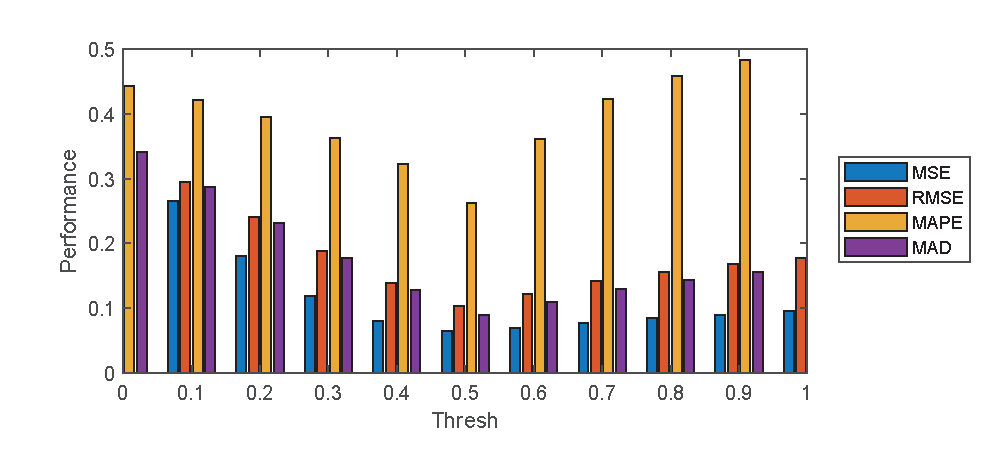
\includegraphics[width=\linewidth]{figs/thresh.eps}
\label{fig:thresh}
\end{figure}

\paragraph{Parameter settings}
$\beta$ was adjusted when the impact of positive events was integrated into stress prediction.
For each of the four groups of stress-buffering patterns,
we adjust $\beta$ to the effect of $\beta \times L$.
We calculated the corresponding prediction result for each adolescent as follows,
and showed the result of the entire testing group in the average performance.
Figure \ref{fig:thresh} shows the changing trend under the L\&S\&P pattern.
The prediction errors decreased first and then increased,
and the best performance was achieved when $\beta$ was
approximately 0.52, with an MSE of 0.0649, an RMSE of 0.2548,
a MAPE of 0.2638 and a MAD of 0.0858 as the average performance of the entire experimental dataset.
Multiple methods for integrating the stress-buffering impact of positive events into stress prediction could be adopted in the future.
In this paper,
we adopted a simple method to verify the effectiveness of our model in quantifying the impact of positive events.
The setting of $\beta$ could be changed according to different individuals and datasets.

\section{Discussion}
\label{sec:conclude}
The main contribution of the present study lies in the following three aspects.
%��һ����֤����չ�������о��Ľ������ֻ�������۸����ϣ��������ڸ������Ϊ��
First, we validated and expanded the theoretical results of previous studies.
The characteristics of stress-buffering were not only manifested in self-reported subjective feelings,
but also in behavioral level in social networks.
%���۵Ĵ��£������˻����¼��ķ�����ѹ��״̬�µ������귢��΢����Ϊ��΢�����ݼ�ѹ���仯֮���DZ�ڹ�����ϵ������֤�˻����¼���ѹ���������÷ֱ������ڼ���ǰ�ڵ�ѹ�����ߺͼ��ٺ��ڵ�ѹ�����������档���о������
We examined the potential relationship between the occurrence of positive events and the posting behaviors,
microblog contents and stress change mode on stressed adolescents,
and verified that
positive events buffered monotonous stress changes at both the early and late stages.
%�ڶ�������ʵ���˷����ϵĴ��¡����о����һ�������ļ�����ܣ�ʵ����1������΢�������Զ���ȡ�����¼����û���Ϊ������2������������Ϊ��������ǰ�����¼������µ�΢����Ϊģʽ��3������ģ��ʵʱ����������ѹ��������̡�
Second, this study implemented the innovation of methods.
Through building a complete technical framework,
we realized
1) automatic extraction of positive events, as well as users' behavior and content measures from microblogs,
and 2) quantification of relationships between stress-buffering of positive events and microblogging measures.
%�������ش���ʵ���壺һ����ʵ���˻���΢����������Դ�����������ѹ���������������ʱ��������⣬�������������������Ŀ�ѹ�ԣ���һ���棬�ɶ�ѧУ�ͼҳ���ʱ���ź��ֻ����¼��Ի���������ѹ���ṩ�������顣
Third, this article showed practical significance.
It realized timely and continuous monitoring of the stress-buffering process
of adolescents based on public social network data sources,
which could be used to assess the stress resistance of adolescents;
on the other hand, it could provide supplementary advice to schools and parents about
'when to arrange positive events to ease stress of adolescents'.

%2
There were three groups of results in this work.
In study 1, the scheduled school events with exact time intervals and the microblogs posted by a group of 500 students were collected and statistically analyzed.
Results showed that when positive events were scheduled neighboring stressful events,
students exhibited less stress intensity and shorter stressful time intervals from their microblogs.
The study also found that most students talked less about the upcoming or just-finished exams when positive events happened nearby,
with lower frequency and lower ratio.
The results substantiated previous studies reporting the protective effect of positive events on adolescents~\citep{Cohen2010Positive,Shahar2002Positive} using laboratory methods.
Based on this, this article carried out more in-depth follow-up studies.

The second groups of results were presented in study 2,
examining stress-buffering pattern of positive events through microblog content and behavioral measures.
As basis, a complete solution was provided for automatically detecting positive events based on microblog semantics,
which were totally different from traditional questionnaire methods,
enabling timely, fraud-proof and continuous detection.
In order to eliminate the possible errors in positive event detection and avoid false overlays,
we first used four scheduled positive events to examine significant stress-buffering effects.
Results showed the event 'holiday' exhibited the highest proportion of significant stress-buffering.
However, this conclusion was questionable because the frequency of the above four events was different and might affect the experimental results.
Next, the stress-buffering effect of automatically extracted positive events were tested based on three groups of stress-buffering measures.
The most intensive stress-buffering effects were shown in 'school life' and 'peer relationship' dimensions.
\emph{Posting behaviors} exhibited most significant correlations among three groups of measures.
This resonated with the study \cite{BLACHNIO2016664,Disclosure} suggesting that users who
tended to share important news on Facebook had a higher level of stress.

This article proposed a novel perspective to better understand the process of stress-buffering.
Since more complex situations were simplified in the present exploration,
the goals were still salient for stress-buffering researches from social networks.

\section{Limitations and future work}

This study has a number of limitations.
% 1) study 1 �����ݹ۲�����˸����¼�
First, it used the microblog data set collected from social networks of high school students,
and chose the scheduled school events as the ground truth in the pilot study.
This could be seen as a relative fuzzy verification method,
because individual events (i.e., 'lost love', or 'received a birthday present') might also conduct additional impact.
Therefore, the data observation in the pilot study were not 100\% rigorous and needed further verification.
A improvement might be conducted by inviting participants to complete related scales (e.g., positive and stressor scales),
thus to label part of the data set,
and achieve a balance between data volume and accuracy.

% 3) δ���ǵ���Ӱ��
Second,
this study treated positive events as independent existence and studied the effect of each event separately.
This ignored the additive and collective effects of multiple positive events which might happened at the same time.
Thus, our future research might investigate the overlap effects of multiple positive events,
as well as the frequent co-appearing patterns of different types of positive events,
thus to provide more accurate stress-buffering guidance for individual adolescents.
%: 1) personality, 2) social support

Based on current research implications,
more factors could help analyze stress-buffering patterns among adolescents more comprehensively in future research.
One factor is how personality ~\citep{personality1,personality2} impacts the stress-buffing effect of positive events,
which could be captured from the social media contents.
Another key factor is the role the social support~\citep{socialSupport1, socialSupport2} in social networks plays.
This factor leaves clues in the messages under each post,
and the behaviors (i.e., retweet, the like numbers) of friends.
For examples, ~\citep{socialSupport1} showed that the number of Facebook friends was associated with stronger perceptions of social support,
which in turn correlated with reduced stress and greater well-being.
The corresponding experimental design, and the online-offline complementary verification will be challenges in the future work.
%��������������»��׼ȷ�����Ǵ�������������ִ�У���Ч���Զ���Ƿ�����Ҫ�����̽����

%\section*{References}

\section{Reference}
\bibliographystyle{model4-names}
\bibliography{reference-new}
\end{document}
